\section{Network Slicing} \label{sota:slicing}

\later{add NSaaS somewhere}

\acs{5G} networks have been regarded by the industry and academia as a critical advancement in the support of next generation vertical applications, tailored to different service requirements and characteristics. This capability is accomplished through network slicing, which allows the creation of \acs{E2E} logical networks (network slices) on a common underlying infrastructure. Network slices are  self-contained, mutually isolated, independently managed and controllable to support programmable multi-service and multi-tenancy environments on a shared infrastructure~\cite{slicingUsingSdnNfvTaxonomy}.

Network Slices support a variety of services, expanding the traditional \acs{5G} service types introduced earlier (\acs{eMBB}, \acs{URLLC} and \acs{mMTC}) into a standardized set of \acf{SST} values, with \acs{SST} values 1,2,3,4,5 and 6 corresponding to \acs{eMBB}, \acs{URLLC}, \acs{mMTC}, \acf{V2X}, \acf{HMTC} and \acf{HDLLC}, respectively~\cite{ETSI_TS_123_501_V16_9_0}. 

\subsection{Network Slice Design \& Instance Lifecycle} \label{sec:slice:lifecycle}

The \acf{GST} by \acs{GSMA} provides a standardized list of attributes that characterize the different types of network slices and, consequently, of services. However, it is designed to be generic, not tied to any specific type of network slice or agreement between a \acf{NSC} and a \acf{NSP}. The \acs{GST} serves as the baseline for creating \acfp{NEST}, with specific values being assigned to the \acs{GST} to express a given set of requirements and support a network slice customer use case~\cite{GSMA_GST}. 

\acsp{NSP} can build their network slice product offerings based on \acsp{NEST}, encapsulating the concrete performance characteristics offered to the customer, which facilitates the establishment of \acfp{SLA} between operators and verticals and fosters interoperability. More specifically, \acsp{NEST} are the foundation for the \acs{NSP} deployment of a network slice, representing the initial step in the \acf{NSI} lifecycle, i.e. network slice preparation~\cite{GSMA_GST}.

\begin{figure}[H]
    \centering
    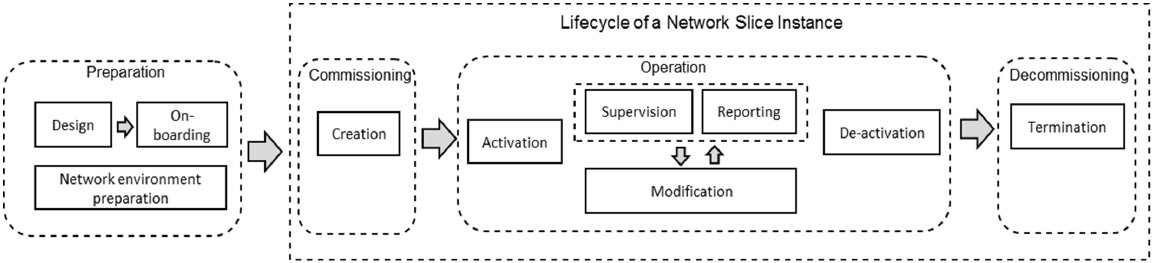
\includegraphics[width=1\linewidth]{figs/NSI_lifecycle.png}
    \caption{\acs{NSI} Lifecycle~\cite{ETSI_MANAGEMENT_ORCHESTRATION_CONCEPTS}}
    \label{fig:slicing:NSI_lifecycle}
\end{figure}

The \acs{NSI} encompasses the full set of Network Function instances and the required resources (e.g. compute, storage and networking resources) of a deployed Network Slice~\cite{ETSI_TS_123_501_V16_9_0} and its corresponding lifecycle is composed by the following phases highlighted in Figure \ref{fig:slicing:NSI_lifecycle}~\cite{ETSI_MANAGEMENT_ORCHESTRATION_PROVISIONING,ETSI_MANAGEMENT_ORCHESTRATION_CONCEPTS}:

\begin{itemize}
    \item \textbf{Preparation:} At this stage, the \acs{NSI} does not yet exist. The \acs{NEST} is created, verified, and onboarded during this phase. It also includes, apart from network slice design, the on-boarding and evaluation of the network functions and all necessary preparations (e.g. network preparations) required before the creation of a \acs{NSI};

    \item \textbf{Commissioning:} The \acs{NSI} is created, which involves allocating and configuring all required resources to satisfy the network slice requirements;
    
    \item \textbf{Operation:} This phase includes the activation, supervision and reporting (related to performance, such as \acs{KPI} monitoring), resource capacity planning, modification and deactivation. The first activates the \acs{NSI}, making it ready to provide communication services, whereas the latter does the opposite. Resource capacity planning involves any actions that calculate resource usage based on \acs{NSI} provisioning and performance monitoring, deriving modification polices as a result of the calculation. \acs{NSI} Modification may be triggered by receiving new network slice requirements or as the result of supervision/reporting and it includes the creation or modification of the \acs{NSI} constituents. Capacity or topology changes correspond to examples of a \acs{NSI} modification;
    
    \item \textbf{Decommissioning:} Encompasses the decomissioning of the required non-shared constituents and the removal of the \acs{NSI} configuration from the shared constituents, after which the \acs{NSI} is terminated and ceases to exist.

\end{itemize}


\subsection{Network Slice Management Functions}

For the purpose of \acs{NSI} management, the concept of a \acf{NSS} is introduced. As outlined in Figure \ref{fig:slicing:class:diagram}, a \acs{NSS} represents a group of network functions (physical and/or virtualized) and their corresponding resources that form part or all of the constituents of a network slice. A \acs{NSS} may be shared between multiple other network slices or subnets and contain instances of \acf{CN} and/or \acf{AN} network functions. Additionally, it may also specify the \acf{TN} requirements necessary to support connectivity between the \acs{CN} and the \acs{AN} network functions within the network slice subnet, covering \acs{TN} topology requirements and individual \acs{TN} links' \acs{QoS} attributes requirements~\cite{ETSI_MANAGEMENT_ORCHESTRATION_CONCEPTS}.

The instantiation of a \acs{NSS} results in a \acf{NSSI}. Similarly, an \acs{NSI} may be composed of one or more \acsp{NSSI} that abide by the same constraints defined for the \acs{NSS} throughout this paragraph. For instance, instantiating an \acs{NSI} with \acs{RAN} and \acs{CN} components may entail defining each domain's component as a separate \acs{NSSI}, potentially shared across multiple \acsp{NSI}~\cite{3GPP-28.801}. Both these constructs must therefore be managed and coordinated correctly to ensure the correct operation of a network slice. 

\begin{figure}[H]
    \centering
    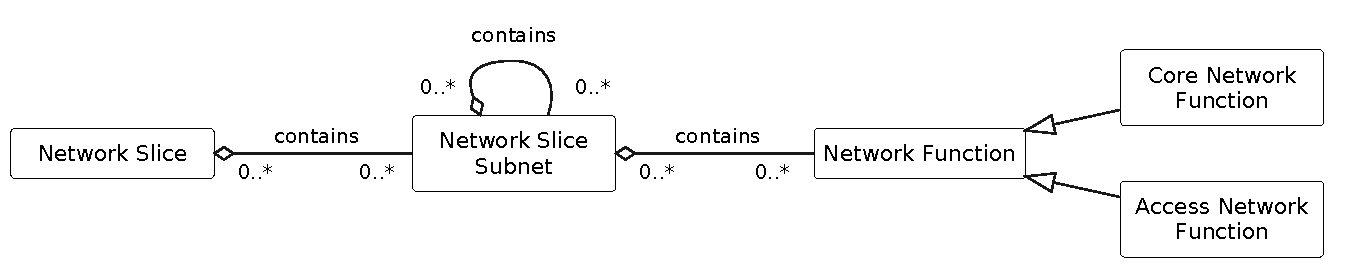
\includegraphics[width=1\linewidth]{figs/plantuml/network-slice-class-diagram.pdf}
    \caption{Network Slice Information Model~\cite{3GPP-28.801}}
    \label{fig:slicing:class:diagram}
\end{figure}

This section identifies three management functions involved in the management and orchestration of network slicing and, consequently, in the support of communication services: the \acf{CSMF}, the \acf{NSMF} and the \acf{NSSMF}. These management functions are organized in a hierarchical structure, where each function delegates part of the related procedures to the next function immediately after it, as showcased in Figure \ref{fig:slicing:management_functions}.

\begin{figure}[H]
    \centering
    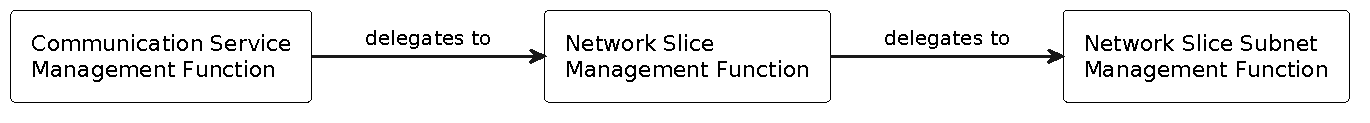
\includegraphics[width=1\linewidth]{figs/plantuml/network-slice-mgmnt-func.pdf}
    \caption{Network Slicing Management Functions~\cite{3GPP-28.801}}
    \label{fig:slicing:management_functions}
\end{figure}

The \acs{CSMF} is responsible for managing the communication services offered by an operator, receiving the requirements requested by end-customers and translating them into concrete network slice requirements, such as network type, network capacity and \acs{QoS} requirements~\cite{3GPP-28.801}. This functionality is closely aligned with that of an \acs{OSS}/\acs{BSS}, which will be further discussed in Section \ref{sota:bss-oss-mano}. These requirements are then forwarded to the \acs{NSMF}, which handles the management of \acsp{NSI} based on the provided requirements. Lastly, the \acs{NSMF} converts the network slice requirements to network slice subnet requirements, which are subsequently delegated to the \acs{NSSMF} for managing and orchestrating \acsp{NSSI}~\cite{3GPP-28.801}.

The management of network slices using these management services must span across the various parts of the network, including both \acs{3GPP} managed network components, such as the \acs{CN} and \acs{AN}, as well as non-\acs{3GPP} components. With this goal, the \acs{3GPP} management system derives each domain's requirements from the customer's service requirements (for a given communication service) and forwards them to the corresponding domain management systems, coordinating the exchange of data between them. For components outside the \acs{3GPP} domain, such as the \acs{TN}, this implies coordinating with the corresponding external management systems to communicate the network slice requirements~\cite{ETSI_MANAGEMENT_ORCHESTRATION_CONCEPTS}.

This is especially relevant, not only in the context of the \acs{TN}, but also considering the inherent virtualization nature of network slicing. When an operator wants to create a network slice, i.e. a \acs{NSI} that includes virtualized network functions, the \acs{NSSMF} should, per request from the \acs{NSMF}, create the needed \acsp{NSSI}, according to the network slice requirements. This involves coordinating with an external management system, namely the \acs{NFV-MANO}, to instantiate and configure all \acsp{VNF} and \acsp{NS}, scaling them as needed for the operations of the \acs{NSI}, while accounting for the fact that these resources may be shared by multiple \acsp{NSSI}. Only after coordinating with the \acs{NFV-MANO}, and performing the necessary application level configurations to the \acsp{NF} allocated to the \acs{NSSI}, the \acs{NSMF} can proceed with the activation of the \acs{NSI}~\cite{3GPP-28.801}.

\subsection{Network Slice Managers}

A Slice Manager is a software system that allows the orchestration and lifecycle management of network slices. The following section presents an overview of two slice managers: the Katana Slice Manager and \acs{ITAv}'s Slice Manager.

\subsubsection{Katana Slice Manager}

Katana is a slice manager solution developed as a part of the 5GENESIS project~\cite{KatanaSliceManagerGenesis}. Through its \acf{NBI}, it receives the \acs{NEST} for creating the network slices, providing an \acs{API} for managing and monitoring them. The \acs{NEST} descriptor, specified in \acs{YAML} or \acs{JSON}, specifies the network slice characteristics and parameters, including \acs{NFV} components, \acs{QoS} monitoring level and Life-Cycle stages. Based on the onboarded \acs{NEST}, the slice manager maps the available data plane resources to the described slice requirements in order to create the requested slice. Additionally, the slice manager communicates with the components from the Management Layer through its \acs{SBI}, including the \acf{VIM}, \acf{NFVO}, \acf{EMS} and \acf{WIM}.

To accommodate multi domain testbed environments, it was developed as a standalone solution that interacts with other components of the \acf{MANO} layer via the defined interfaces (e.g. through SOL005 interface for \acf{OSM} \acf{NFVO}), as to allow the management of the network slice's lifecycle without extended \acs{MANO} functionality~\cite{KatanaSliceManagerGenesis}

\begin{figure}[H]
    \centering
    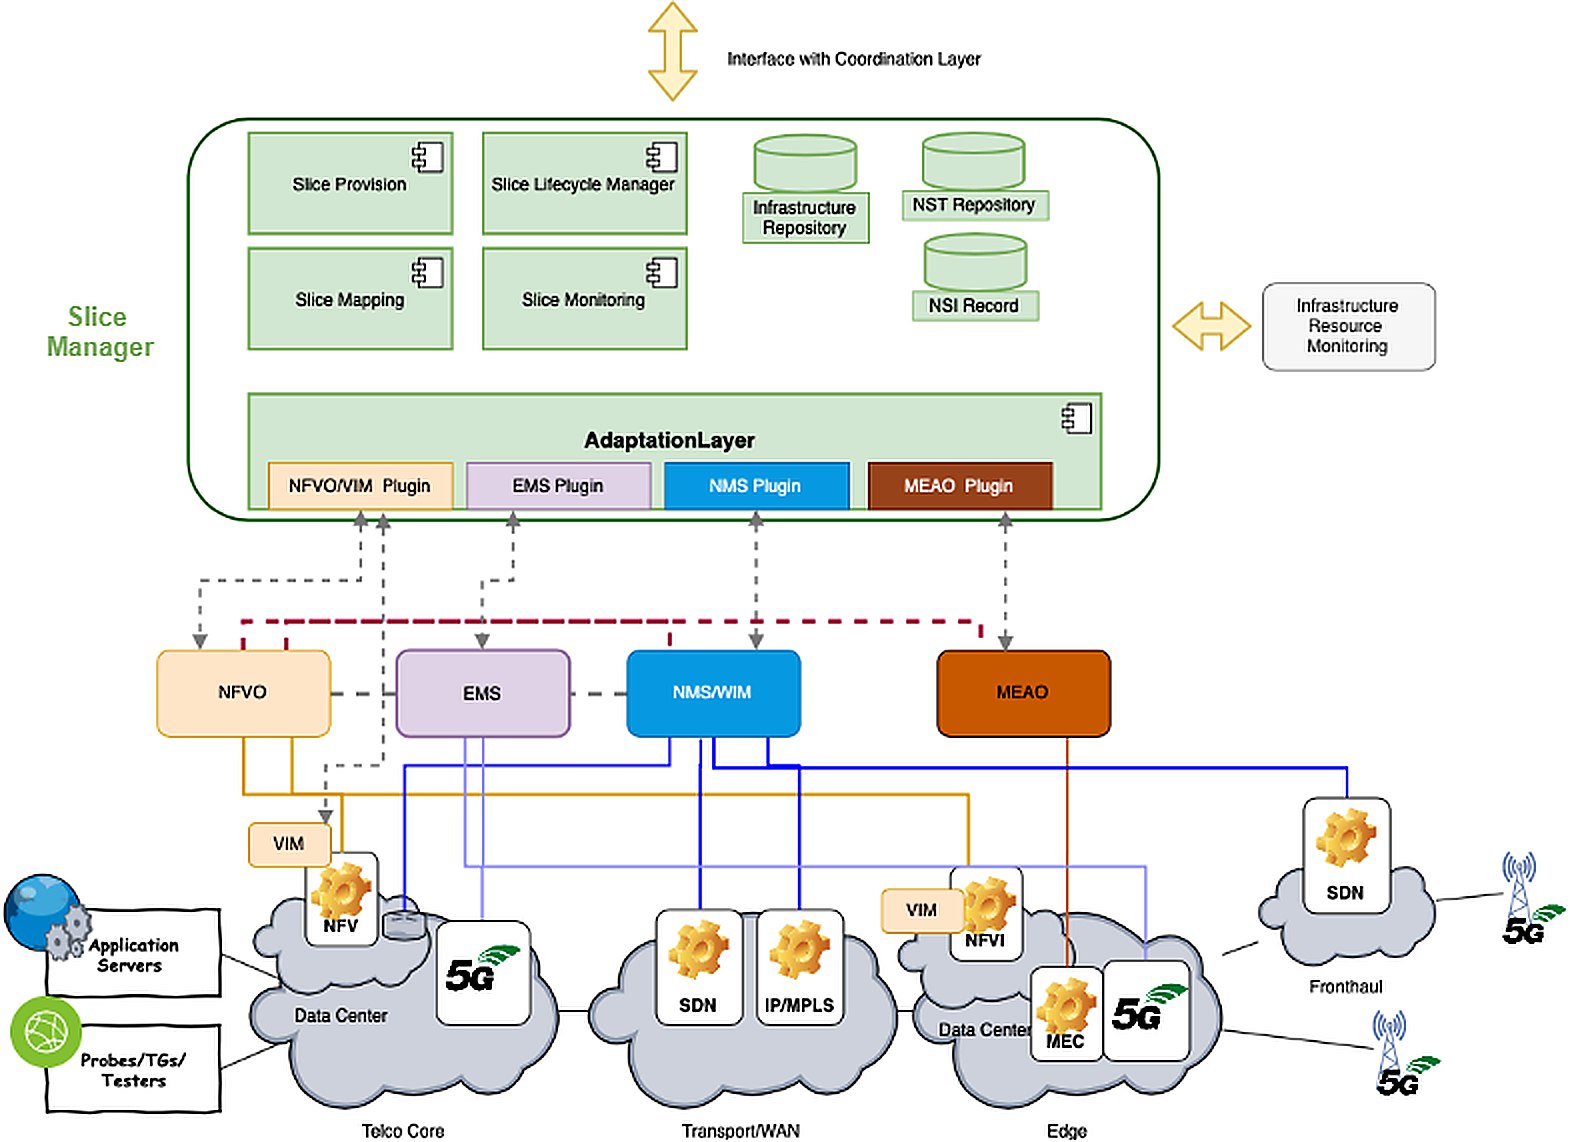
\includegraphics[width=0.95\linewidth]{figs/katana-architecture-upscaled.png}
    \caption{Katana Slice Manager Architecture~\cite{KatanaSliceManagerWiki}}
    \label{fig:katana:architecture}
\end{figure}


The Katana Slice Manager follows a highly modular architecture, implemented as a mesh of independent microservices, each running in a dedicated Docker container. Figure \ref{fig:katana:architecture} illustrates the architecture of the slice manager, highlighting its constituent modules and their interconnections, as described bellow~\cite{KatanaSliceManagerWiki}.

\customparagraph{North Bound Interface API}

The \acf{NBI} provides a set of \acs{REST} \acsp{API}, to be consumed by a component of the coordination layer, such as the Experiment Lifecycle Manager. It includes two submodules that consume these \acs{REST} \acsp{API}, allowing a user or admininstrator to interact with it: (i) a \acf{CLI} for Bash commands interaction via the terminal and a (ii) web \acf{GUI} that interacts with the Slicing Lifecycle Manager and repositories to create new slices. 

\customparagraph{Slicing Lifecycle Manager}

This module serves as the central component of the slice manager, responsible for managing the lifecycle of network slices through \acs{CRUD} operations. It handles requests from the \acs{NBI} \acsp{API} and executes the required actions to activate, modify or deactivate a network slice. Additionally, it receives status updates from the Slice Monitoring module regarding a given slice, coordinating with other components to trigger the appropriate processes in response to these changes. Lastly, it is also tasked with optimally selecting the infrastructure resources to be used for a new slice, according to the available resources and the slice requirements, during the slice creation phase.

\customparagraph{Slice Mapping}

The Slice Mapping component manages the slice mapping process, following the request for a new slice. It maps the \acs{GST} requests with a specific \acs{NEST} that is supported by the infrastructure.

\customparagraph{Slice Provisioning}

Receives requests from the Slicing Lifecycle Manager service to setup, configure or delete \acs{WAN} paths, isolated \acs{NFVI} tenant spaces and the related network services. It also manages the configuration of radio component parameters and the registration of the newly created slice into the Monitoring system. All of the aforementioned functionalities are achieved by utilizing plugins of the Adaptation Layer.

\customparagraph{Slice Monitoring}

This module is responsbile for monitoring the health and the status of every deployed slice. Similarly to the previous service, it relies on Adaptation Layer plugins to send status check messages to the \acs{MANO} components and report status changes to the Slicing Lifecycle Manager.

\customparagraph{Adaptation Layer}

The Adaptation Layer provides an abstraction layer over the underlying technology, allowing the slice manager to operate over any \acs{MANO} layer component without any modifications to its core functionality, given the correct plugin is installed. This module includes plugins for each of the slice manager's \acs{MANO} layer components, which are responsible for receiving and translating requests from the Slicing Lifecycle Manager into the corresponding component \acs{API}, and, consequently, processing the responses.


This architecture provides the baseline for the provisioning and lifecycle management of network slices. However, the Katana open source project has been inactive, with no updates since December 2022, rendering it unusable for this dissertation. It does not support more recent \acs{OSM} versions, with the latest compatible release being \acs{OSM} 8.


\subsubsection{ITAv Slice Manager}

\acf{ITAv} has its own proprietary implementation to automate the deployment and management of network slices in \acs{5G} networks~\cite{ITAvSliceManager}. The \acs{ITAv} Slice Manager is currently deployed on the 5GAIner testbed~\cite{5GAIner}, a commercial-grade \acs{5G SA} infrastructure also available at \acs{ITAv}. The solution enables the programmatic reconfiguration of the \acs{5G} network, provisioning slices tailored to meet the requirements of the three primary \acs{5G} services: \acs{eMBB}, \acs{URLLC} and \acs{mMTC}/\acs{MIoT}. The slices configured by the network slice manager preserve the network \acf{TRL}, being the produced
slices representative of a commercial-graded solution. Moreover, the slice manager also offers dynamic slicing capabilities, supporting the adaptation of the slice performance in real time without communication disruption.

The \acs{ITAv} Slice Manager is designed with a strong focus on adherence to established standards to ensure interoperability and seamless interaction with other software systems, as defined by \acs{3GPP}. In particular, it complies with the following specifications:

\begin{itemize}
    \item 3GPP TS 28.531 version 18.3.0~\cite{ITAv_3gpp_28531_v18_3_0}: outlines the essential Network Functions for a standardized network slice manager;
    
    \item 3GPP TR 28.824 version 18.1.0~\cite{ITAv_3gpp_28824_v18_0_1}: identifies the \acf{TMF} standards required for the Slice Manager, with adherence to TMF622\_ProductOrder~\cite{TMF622UserGuideV5} and TMF641\_ServiceOrder~\cite{TMF641UserGuideV411}, as defined in December 2023;

    \item 3GPP TS 28.541 version 18.4.1~\cite{ITAv_3gpp_28541_v18_4_1}: delineates the profiles associated with network slices (e.g. ServiceProfile, TOPSliceSubnetProfile);

    \item 3GPP TS 28.530 version 17.4.0~\cite{ITAv_3gpp_28530_v17_4_0}: presents the Network Slice Management Lifecycle.
\end{itemize}

According to the original work~\cite{ITAvSliceManager}, the \acs{ITAv} Slice Manager supports an extensive list of Slice Manager requirements identified throughout the literature: \ac{E2E} Slice Support, Slice Lifecycle Management, Network Configuration, Policy and \acs{QoS} Management for \acs{SLA} Enforcement, Dynamic Slicing, Custom Slices, Network Slice Monitoring, Location-based Slicing, Performance Assurance, Multiple Slice Management, Network Resource Monitoring, Slice Feasibility Evaluation, and Generic Network Support. Furthermore, the slice manager solution can be integrated with \acs{OSM} and \acf{OSL}, allowing adherence to an even more complete set of requirements with orchestration and \acf{OSS} capabilities~\cite{ITAvSliceManager}. The \acs{ITAv} Slice Manager represents a significantly more mature solution than the available alternatives.


